\documentclass[preprint,11pt,3p]{elsarticle} %review, or preprint

\usepackage{amssymb}
\usepackage{graphics}
\usepackage{float}

\usepackage{color}
\usepackage{lscape}

\usepackage[toc,page]{appendix}

%For tracking changes
\usepackage{changes}
\definechangesauthor[name={Prageeth}, color=orange]{pj}
\definechangesauthor[name={Zoltan}, color=blue]{zoltan}
\definechangesauthor[name={Johannes}, color=cyan]{johannes}
\definechangesauthor[name={Prageeth2}, color=magenta]{pj2}
\usepackage[normalem]{ulem}

%Flowcharts
\usepackage[latin1]{inputenc}
\usepackage{tikz}
\usepackage{circuitikz}
\usetikzlibrary{shapes,arrows}
\tikzstyle{decision} = [diamond, draw, 
    text width=4.5em, text badly centered, node distance=3cm, inner sep=0pt]
\tikzstyle{block} = [rectangle, draw, 
    text width=6em, text centered, rounded corners, minimum height=3em]
\tikzstyle{line} = [draw, -latex']
\tikzstyle{cloud} = [draw, ellipse, node distance=3cm,
    minimum height=2em]
\tikzstyle{noborder} = [node distance=3cm, text width=6em, text centered, minimum height=2em]

%For subfigure
\usepackage{graphicx}
\usepackage{caption}
\usepackage{subcaption}

%Stop footnote from skipping to next page
\interfootnotelinepenalty=10000

%Some code to display the units after the equation 
\usepackage{mathtools}
\makeatletter
\providecommand\add@text{}
\newcommand\tagaddtext[1]{%
  \gdef\add@text{#1\gdef\add@text{}}}% 
\renewcommand\tagform@[1]{%
  \maketag@@@{\llap{\add@text\quad}(\ignorespaces#1\unskip\@@italiccorr)}%
}
\makeatother



\graphicspath{{./Images/}}

\journal{CISBAT}

%\journal{Solar Energy, Energy and Buildings, Building and Environment, Energy Science and Engineering}

\begin{document}

\begin{frontmatter}

% \begin{figure}
% \begin{center}
% 
\includegraphics[width=\columnwidth, trim= 0cm 0cm 0cm 0cm,clip]{HeaderEP.pdf}
% \label{fig:header}
% \end{center}
% \end{figure}

\begin{center}
{CISBAT 2019 International Conference - Future Buildings \& Districts - Energy Efficiency from Nano to Urban Scale, Lausanne, Switzerland}
\end{center}

\title{The Cozie Clock-Face: a methodology for the in-situ collection of occupant comfort data} 
%Energy Performance of PV modules as Adaptive Building Shading Systems
%Numerical Energy Analysis of PV Modules as Adaptive Building Shading Systems


\author[buds]{P. Jayathissa\corref{cor2}}
    \ead{p.jayathissaa@nus.edu.sg}
\address[buds]{Building and Urban Data Science Group,  Department of Building, Singapore} 
% For whatever reason the affiliation needs to be defined after the authors. Otherwise the numbering gets messed up.

\author[buds]{M. Quintana}
  \ead{matias@u.nus.edu}

\author[buds]{T. Sood}
  \ead{matias@u.nus.edu}


\author[unsw]{N. Narzarian}
    \ead{n.nazarian@unsw.edu.au}
\address[unsw]{University of New South Wales, Australia}

% \author[aut]{Z. Nagy}
%     \ead{nagy@utexas.edu}
% \address[aut]{Intelligent Environments Laboratory, Department of Civil, Architectural and Environmental Engineering,\\ The University of Texas at Austin, USA}


\author[buds]{C. Miller \corref{cor1} }
    \ead{clayton@nus.edu.sg}


\cortext[cor2]{Corresponding author}


\begin{abstract}

A 2012 survey of 52'980 occupants in 251 office buildings found that 50\% of all occupants were dissatisfied with their indoor environment \cite{frontczak2012quantitative}. This dissatisfaction can result in a reduction of work performance \cite{wargocki2007effects} and be a precursor for future health issues \cite{jaakkola1989sick}. \\

Significant progress has been made to improve occupant comfort. On one hand, there is the technological advancement of heating, ventilation and air conditioning systems (HVAC). On the other hand, there are advancements in human-building interaction which enables the local environment to adapt to the needs of the occupant \cite{wang2017state}. These methods however have one fundamental limitation. They assume that all occupants within a building zone share the same comfort preference. In reality, variations in metabolic rates \cite{byrne2005metabolic}, light preferences \cite{galasiu2006occupant}, and noise tolerance [citation required] presents a challenge when attempting to condition a work-space to meet the requirements of all occupants \cite{kingma2015energy}.\\

Rather than tailoring the work-space to the preferences of the occupants, an alternative approach is to match the individual to a work-space. This requires an understanding of the individuals comfort preferences and a recommendation engine that can suggest a comfortable workspace in real time based on building environmental sensor data. 

This paper focuses on the first of these challenges, namely comfort data collection. The state of the art in this field are comfort surveys. Although this works it has three main limitations

\begin{itemize}
  \item The methodology cannot be scaled to large sample sets due to the administrative overhead in preparing these studies.
  \item The studies are often conducted outside of the test subjects natural working environment.
  \item Users suffer from survey fatigue \cite{porter2004multiple} due to the number of data points required to conduct a thorough assessment, and even when willing to participate, they are concerned about how accurate they are responding to them \cite{Clear2018}
\end{itemize}

This paper presents a novel form of occupant comfort data collection, using a wearable health tracker, in this case the Fitbit smartwatch, with 25 million active users \cite{fibit2018}. The application is a simple clock-face where the user can state their comfort preference as a binary input "comfy" or "not comfy". The comfort preferences are mapped to a time series database and linked with sensors that were present in the location of the user at that time.\\

This proof of concept has been launched with a small sample set of 15 users. Each user has been equipped with a Fitbit, and a wearable environmental sensor from the National Singapore Science Experiment \cite{wilhelm2016wearable}. All data is collected in-situ in the user's natural work environment. \\

Next steps in this study involve the development of a work-space recommendation engine. This engine will process the data and give each user a unique comfort profile that can be used to recommend work-spaces in real time. This project, known as SpaceMatch will be launched in 2019 at the National University of Singapore. \\

The clock-face application is available for free download from the Fitbit store for future researchers to conduct their own crowd-sourced comfort studies.

\end{abstract}

\begin{keyword}
Comfort Feedback \sep Data Collection \sep Fitbit \sep Comfort Recommendation \sep Mood Logging
\end{keyword}

\end{frontmatter}

\section{Introduction}
\label{ch:introduction}
% !TEX root = 99_main.tex

In the Ma\={o}ri legends of old, there was a time when the sun would travel quickly across the sky, leaving people without sufficient light and warmth. M\={a}ui, a great hero of the time, observed this discomfort amongst the village and went on a quest to tame the sun. Armed with his magic jawbone of Murirangawhenua and a lot of flax rope, he succeeded in tying down the sun and beating it, until it slowed down to the speeds we have today. What M\={a}ui effectively did was categorise everyone in a one-size-fits-all model, and based on this assumption, took action to change the environment he lived in. 

The way we control our buildings today, is similar to the way that M\={a}ui tamed the sun. We make an assumption of the general population based on a survey of a few people, and change the environment we live in based on these few data points. The issue here is that we assume that all occupants within a building zone share the same comfort preferences. In reality, variations in metabolic rates, light preferences, and noise tolerances presents a challenge when attempting to condition a work space to meet the requirements of all occupants. 

However understanding the preferences of individuals presents a significant challenge, both the times of M\={a}ui and now. The state of the art of human comfort data collection is in the form of surveys, either as an online form, or paper based. While this in principal works, it presents three major challenges.

% %A recent survey of 52'980 occupants in 251 office buildings found that 50\% of all occupants were dissatisfied with their indoor environment. 


% From the times of M\={a}ui till now, a significant challenge is the acquisition of human comfort feedback data. The state of the art, in attaining human feedback are surveys, either as an online form, or paper based. 

\begin{itemize}
  \item The methodology cannot be scaled to large sample sets due to the administrative overhead in preparing these studies.
  \item The studies are often conducted outside of the test subjects natural working environment.
  \item Users suffer from survey fatigue \cite{porter2004multiple} due to the number of data points required to conduct a thorough assessment. Even when willing to participate, there is a concern about how accurately their responses are \cite{Clear2018}.
\end{itemize}



This paper presents cozie, a publicly available clock-face designed for fitbit which can be used for tailored, scalable, in-situ human comfort studies. We will show how the watch-face can be deployed for a range of tailored experimental scenarios, and be evaluated using modern data analytics to infer behavioral patterns of the test participants. This information can be used to optimise human comfort through spatial recommendation, or combined with building sensor data to create a labeled data-set for the comfort optimisation of the building management system. \\

% combined with building sensor data to create a high quality labeled data set. 


%  that can be used to optimise the comfort of the user through spatial recommendation, and provide input training data for the comfort optimisation of the building management system.\\

The remainder of the paper is organised as follows. The next section outlines the cozie clock-face and how research teams can implement it for a variety of human comfort related experiments. In Section 3 we detail a preliminary experiment conducted using the cozie clock-face for building comfort optimisation, Section 4 presents the preliminary results from this experiment, and Section 5 discusses our findings and next steps in this project. Finally, Section 6 concludes the paper. 




% \begin{figure}
% \begin{center}
% \includegraphics[width=8cm, trim= 0cm 0cm 0cm 0cm,clip]{facadeFunctionsnew.pdf}
% \caption{The facade acting as a mediator between the interior and exterior environment, while fulfilling various functions \cite{nagy2016adaptive}}
% \label{fig:ASFschematic}
% \end{center}
% \end{figure}

% \begin{figure}
% \begin{center}
% \includegraphics[width=8cm, trim= 0cm 0cm 0cm 0cm,clip]{honr.jpg}
% \caption{An example of an ASF constructed at the House of Natural Resources \cite{nagy2016adaptive}}
% \label{fig:HoNR}
% \end{center}
% \end{figure}






\section{The cozie watch-face}
\label{ch:cozie}
% !TEX root = 99_main.tex

Cozie is built as a clock-face for fitbit, a wearable health tracker with 25 million active users \cite{fibit2018}. The application is publicly available for download at the following link [insert link]

\subsection{Overview}

In this section we define "user" as the test participant who is wearing the fitbit, and "manager" as the person coordinating the experiment. \ 

The default status of the clock-face is a simple binary question: "Comfy" or "Not Comfy", as seen in Figure \ref{fig:homescreen}. By simply clicking one of the icons, information about the users location (GPS), heart-rate, steps walked since last log, and the comfort data is anonymously sent to an Influx time series cloud database [Ref influx]. Data from this database can be simply queried with an API key that can be provided to the manager. Further documentation can be found on the cozie website [insert link].\\

If the manager is interested as to why the user is feeling discomfort, then there is a range of additional questions that can be configured using the cellphone that the fitbit is paired with. The optional questions include: thermal preference, light preference, noise preference, indoor/outdoor, mood, and whether the user is in office. These settings, along with a unique user-id for each user, and a unique experiment-id can be configured by the manager using the cellphone that the fitbit is paired with. The watch-face also has the ability to prompt the user and force them to provde feedback at custom intervals set by the manager.

% \begin{itemize}
%   \item Thermal: Prefer Warmer - Prefer Cooler
%   \item Light: Prefer brighter - Prefer Dimmer
%   \item Noise: Prefer Louder - Prefer Quieter 
%   \item Mood: Good - Neutral - Not So Good
%   \item Location: Indoor - Outdoor
%   \item Location: In Office - Out of Office
% \end{itemize}

%These responses will be grouped with the afore mentioned data, and stored in the Influx time series database. The manager is invited to contact the authors if they have further tailored questions that they would like to add.\\

%The watch-face also has the ability to prompt the user with a 3 second vibration, and force them to provide comfort feedback. This may be triggered at certain hours of the day, random hours of the day, at set time intervals, or at each 1000 steps walked. 

% \begin{figure}
%     \begin{subfigure}[t]{0.3\textwidth}
%         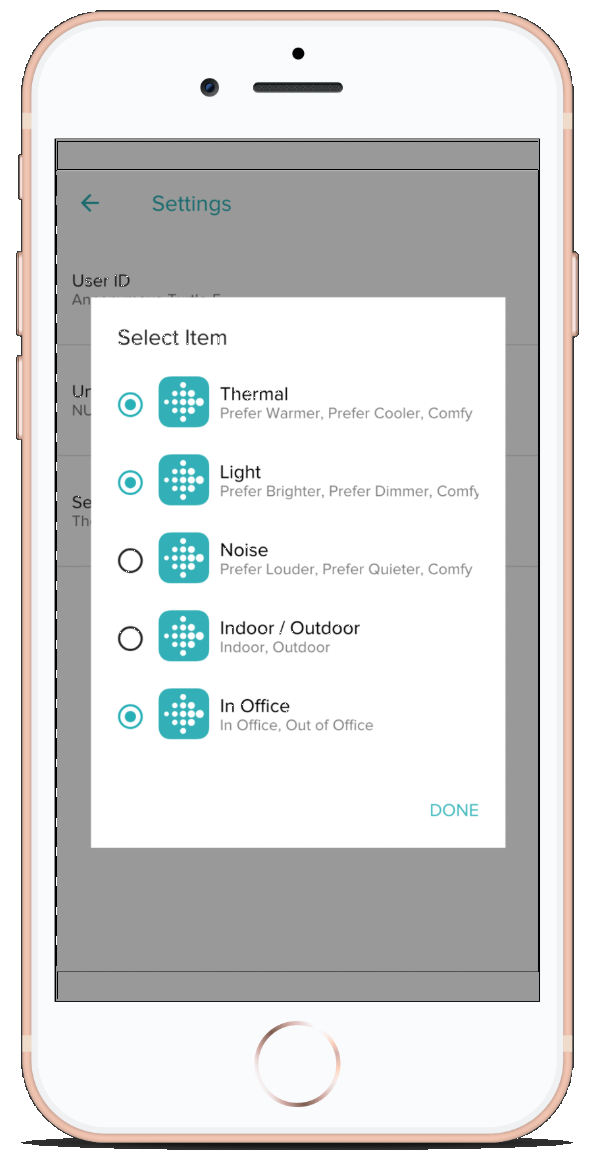
\includegraphics[height= 7cm]{iphone.png}
%     \end{subfigure}
%     \begin{subfigure}[t]{0.3\textwidth}
%         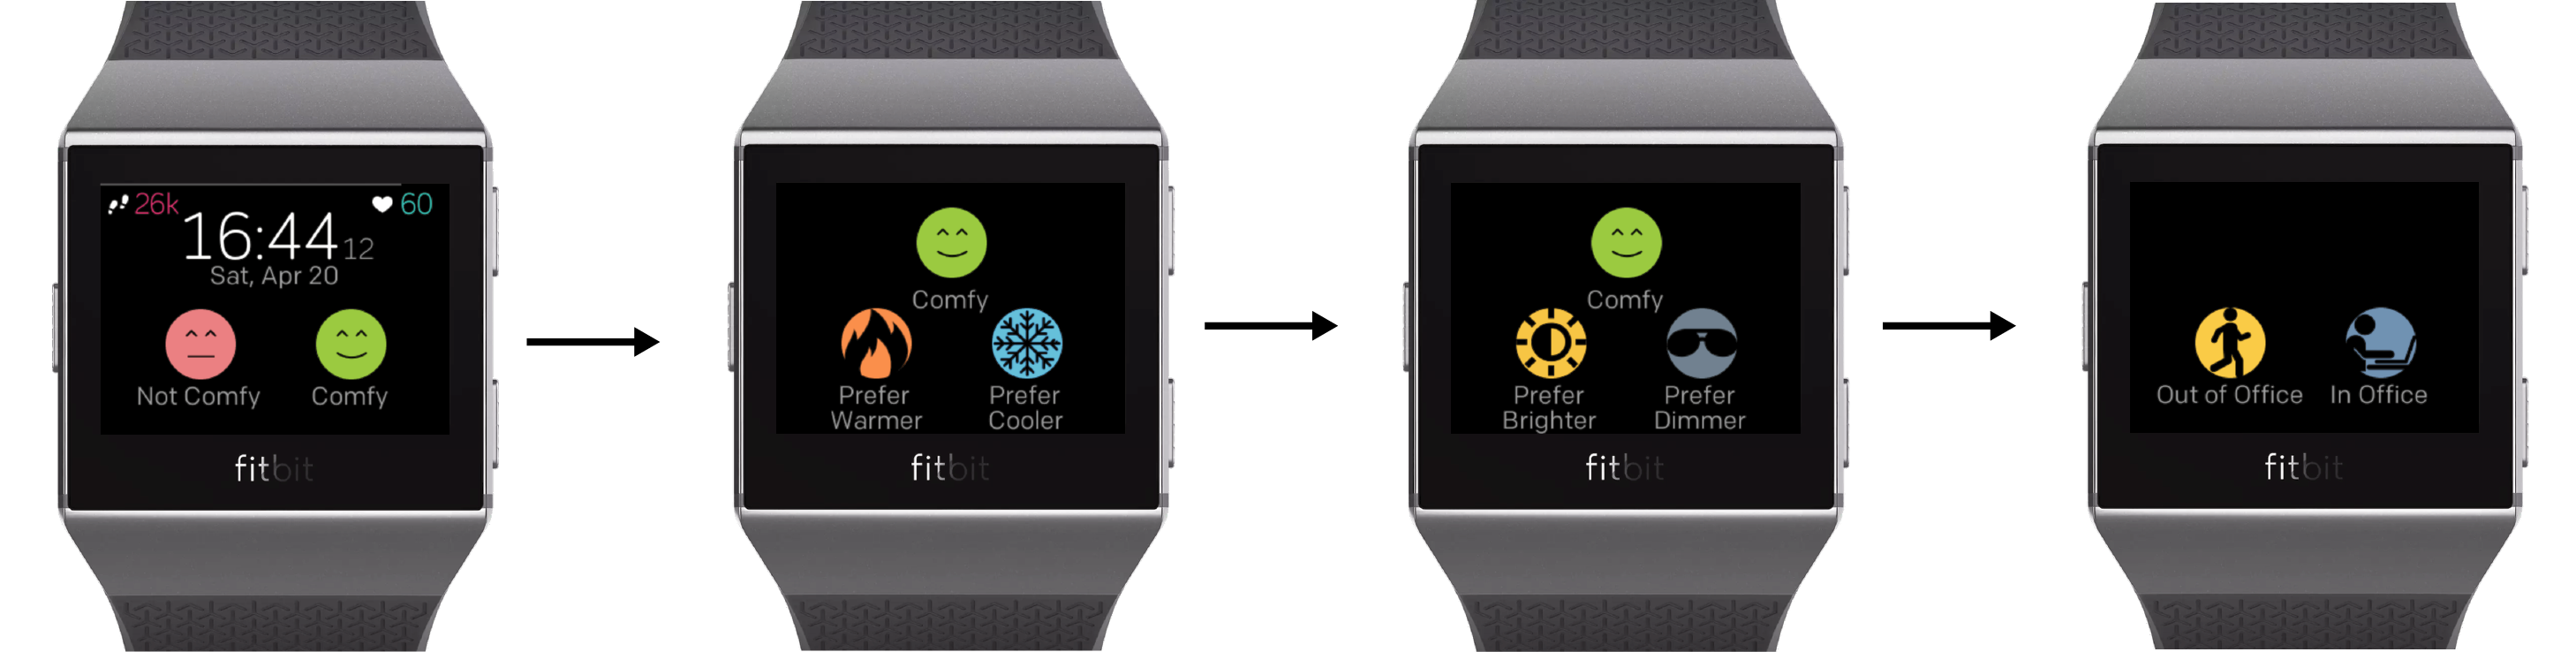
\includegraphics[height= 3cm]{flow.png}
%     \end{subfigure}
%     \caption{Using the fitbit mobile application to design a survey flow}
%     \label{fig:homescreen}
% \end{figure}




% \subsection{Building Data Labeling}

% The human comfort feedback can be combined with building sensor data to create a labeled data set of the environment. (perhaps talk more or delete this section)

% An example of this in practice will be introduced in the next section.

\section{Methodology}
\label{ch:method}
% !TEX root = 99_main.tex

An experiment was deployed as part of \emph{Project Coolbit}\footnote{\url{http://www.projectcoolbit.com}}, an international effort that focusses on the use of smartwatches for human comfort analysis \cite{nazarian2019geophysics}. Fifteen participants residing in Singapore were recruited for the experiment and were equipped with Fitbit Versa or Ionic watches. Most of the participants were working at the National University of Singapore (NUS) at several flexible workspaces around campus.  The \emph{cozie} clock-face was set to request thermal preference (prefer warmer, prefer cooler, comfy), and the set to request feedback at the hours of 9:00, 11:00, 13:00, 15:00, and 17:00. 
%These feedback requests take the form of a gentle vibration of the watch to prompt the user to provide feedback.
% at the hours of 9:00, 11:00, 13:00, 15:00, and 17:00. 

The watch was further complemented with Internet-of-Things (IoT) connected on-body and environmental sensors. The on-body sensor consists of a temperature and light sensor from \emph{mbient-labs}\footnote{\url{https://mbientlab.com/}} that had been modified to fit the watch strap with a custom 3D printed case. An off-body sensor measuring temperature and humidity was attached to the participant's bag. The sensors communicate via Bluetooth to Raspberry-Pi gateways that had been positioned throughout the working space. Data from the cozie clock-face and the environmental sensors were aggregated in an Influx cloud time-series database, which served as a platform for data acquisition and fault detection. 
% Source codes can be found here \cite{aurek-data}.


% \begin{figure}
% \begin{center}
% 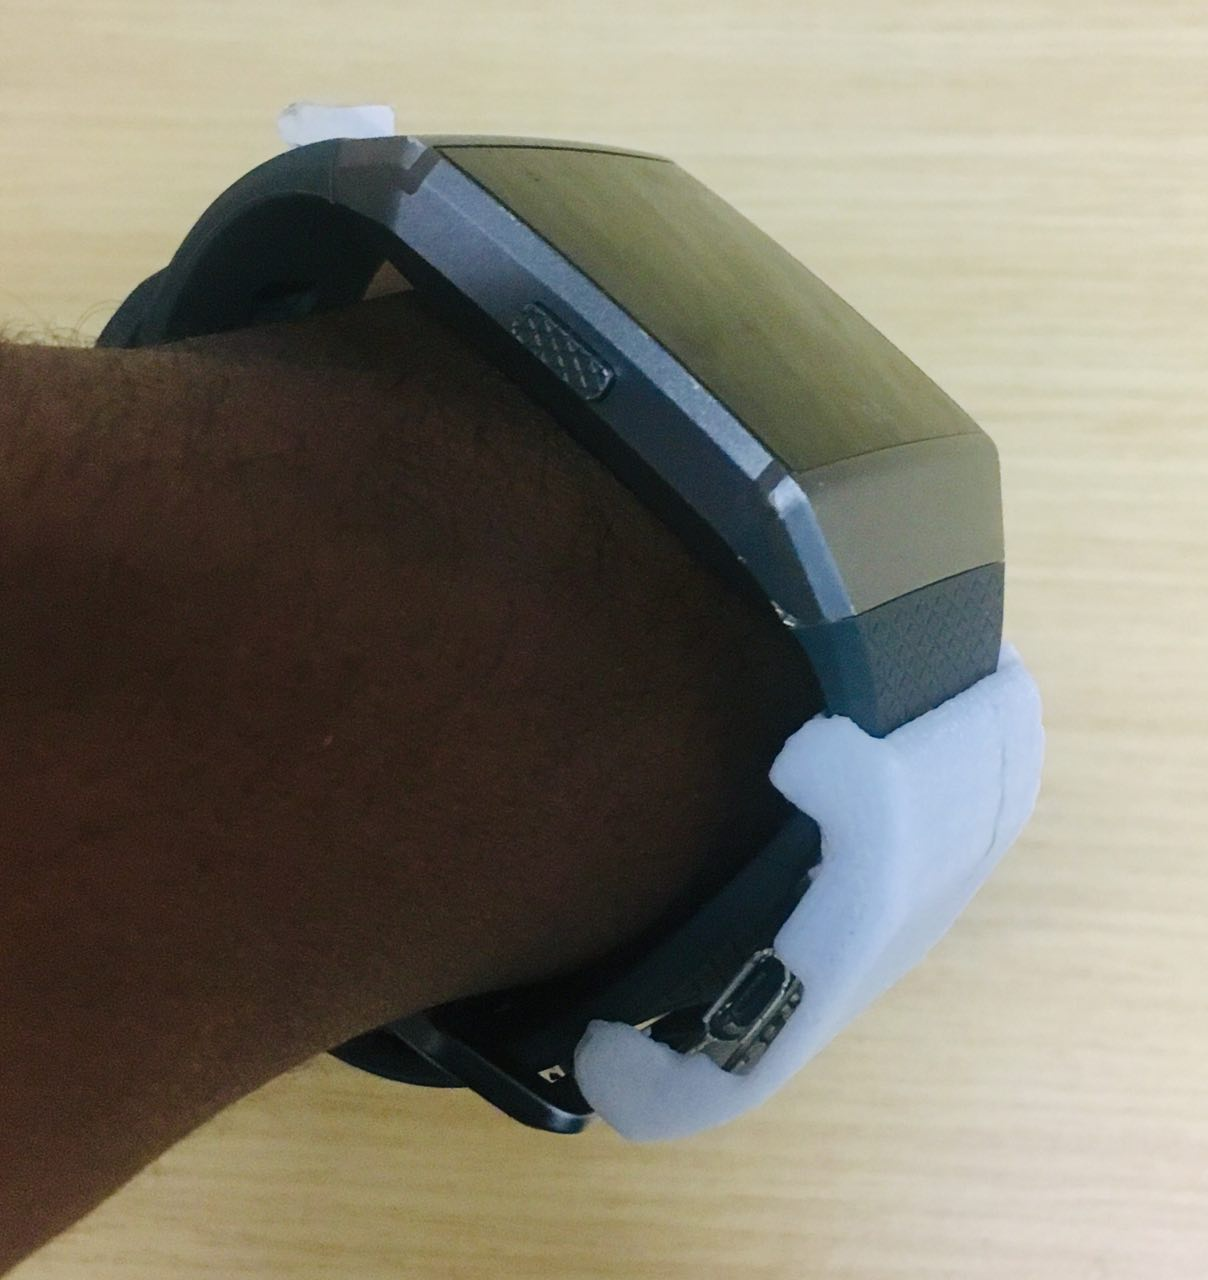
\includegraphics[width=0.2\textwidth, trim= 0cm 0cm 0cm 0cm,clip]{strap-pack.jpg}
% \caption{Strap-Pack}
% \label{fig:strappack}
% \end{center}
% \end{figure}



\section{Results}
\label{ch:results}
% !TEX root = 99_main.tex

The experiment, consisting of fifteen users each equipped with a Fitbit over a month, produced a data set of 1,460 data points. Each data point is effectively a survey of the user at a particular time. The results presented in this section is a demonstration of the type of analysis that can be conducted using data acquired from the \emph{cozie} clock-face.

\subsection{Overview of spatio-temporal data}
Figure \ref{fig:summary}a details the spatial distribution of data throughout Singapore. Each of these data points is tagged with the users heart-rate, response, and local temperature which can be used to infer faults or issues within the building. Figure \ref{fig:summary}b is a simple heat map plotting the number of responses based on the hour of the day, and day of the week. It is interesting to note that 55\% of responses come from the hours of 9:00, 11:00, 13:00, 15:00, and 17:00 when the occupant is buzzed and forced to give feedback. The remaining 45\% of responses are made outside these times through the self-motivation of the participants themselves. Figure \ref{fig:summary}c details the daily responses from the participants, and no observable decrease in responses can be made, indicating no effects of survey fatigue. Dips in responses naturally occur during the weekend, and during the first week when users were still being onboarded. A normal distribution of heart-rate data from the Fitbit heart rate sensor can be found in Figure \ref{fig:summary}d.

\subsection{Merging with environmental sensor data}
Combining the cozie clock-face, with additional environmental sensors opens further dimensions of analysis. User responses are mapped to the environmental condition at which they are exposed, which can provide a high quality labelled data set for training data driven models. Figure \ref{fig:summary}e-f detail the distribution of temperature and humidity data. Unfortunately, due to communication issues from these sensors, not all data points could be recorded. The temperature of the temperature sensor is on average 0.8 $^\circ$C warmer than the surrounding environment due to the influence of body temperature. 

\begin{figure}
\begin{center}
\includegraphics[width=\textwidth, trim= 0cm 0cm 0cm 0cm,clip]{cozie_datasummary.pdf}
\caption{Overview of raw data extracted from the cozie clock-face and additional sensors. (a) spatial distribution of responses throughout Singapore, (b) temporal distribution of responses, (c) number of responses per day over the course of the experiment, (d-f) rug plots detailing the normalised distribution of responses based on the Fitbit heart rate sensor, wrist mounted temperature sensor, and off-body humidity sensor }
\label{fig:summary}
\end{center}
\end{figure}



\subsection{Clustering of thermal comfort personality}
\label{ch:userResults}
Individual user feedback can be clustered using unsupervised learning techniques. In this example, we use a hierarchical k-means clustering based on euclidean distance using the nearest-point-algorithm. The results, shown in Figure \ref{fig:clustering}, show four distinct clusters of users. 
%Users that are comfortable 100\% of the time, users that are comfortable 60-80 \% of the time, those that are comfortable 50\% of the time and generally would prefer it cooler, those that are comfortable 50\% of the time and would prefer it both warmer and cooler. 
Understanding and defining these differences in user preferences can be used to recommend spaces that may better suit the needs of the occupant. For example, Group A, which primarily works off-site can be recommended alternative workspaces that are on average cooler. Group C on the other hand is a single highly satisfied user, who works from a single work-space within a narrow temperature range, and relatively low resting heart-rate. Group D represents our conventional occupant that may be comfortable 70\% of the time. 

Below the cluster plot are spatial distributions of responses that can be used to identify different building climates. The majority of \emph{Prefer Warmer} responses occur in co-working space 1. This area can be labelled as a \emph{cooler working space} for users that would prefer cooler working environments. Alternatively, if facilities management wishes to save energy, increasing the set-point temperature of these \emph{over-cooled} spaces may be a low effort solution which may simultaneously improve occupant well-being. 


%poor building opperation. A large percentage of "prefer warmer" responses appear to occur in co-working space one. Increasing the set-point temperature within this space may improve overall wellbeing, and simultaneously save building energy. Alternatively, this co-working space can 

%It is importat to note that the data is not representative of a single space. As shown in Figure \ref{fig:map}, responses were made throughout Singapore. GPS data can support in localising responses to individual buildings, but also comes with issues which will be discussed in Section \ref{ch:localisation}.


%It is important to note here that the data is not entirely representative of a single building space, as the user may have given feedback while having lunch outside. There are even feedback results made outside of working hours as seen in \ref{fig:hourPlot} \ref{fig:responseRate}. Conclusions such as "Building Zone A was comfortable 80\% of the time" can therefore not be made. This will be further discussed in Section \ref{ch:discussion}.

\begin{figure}
\begin{center}
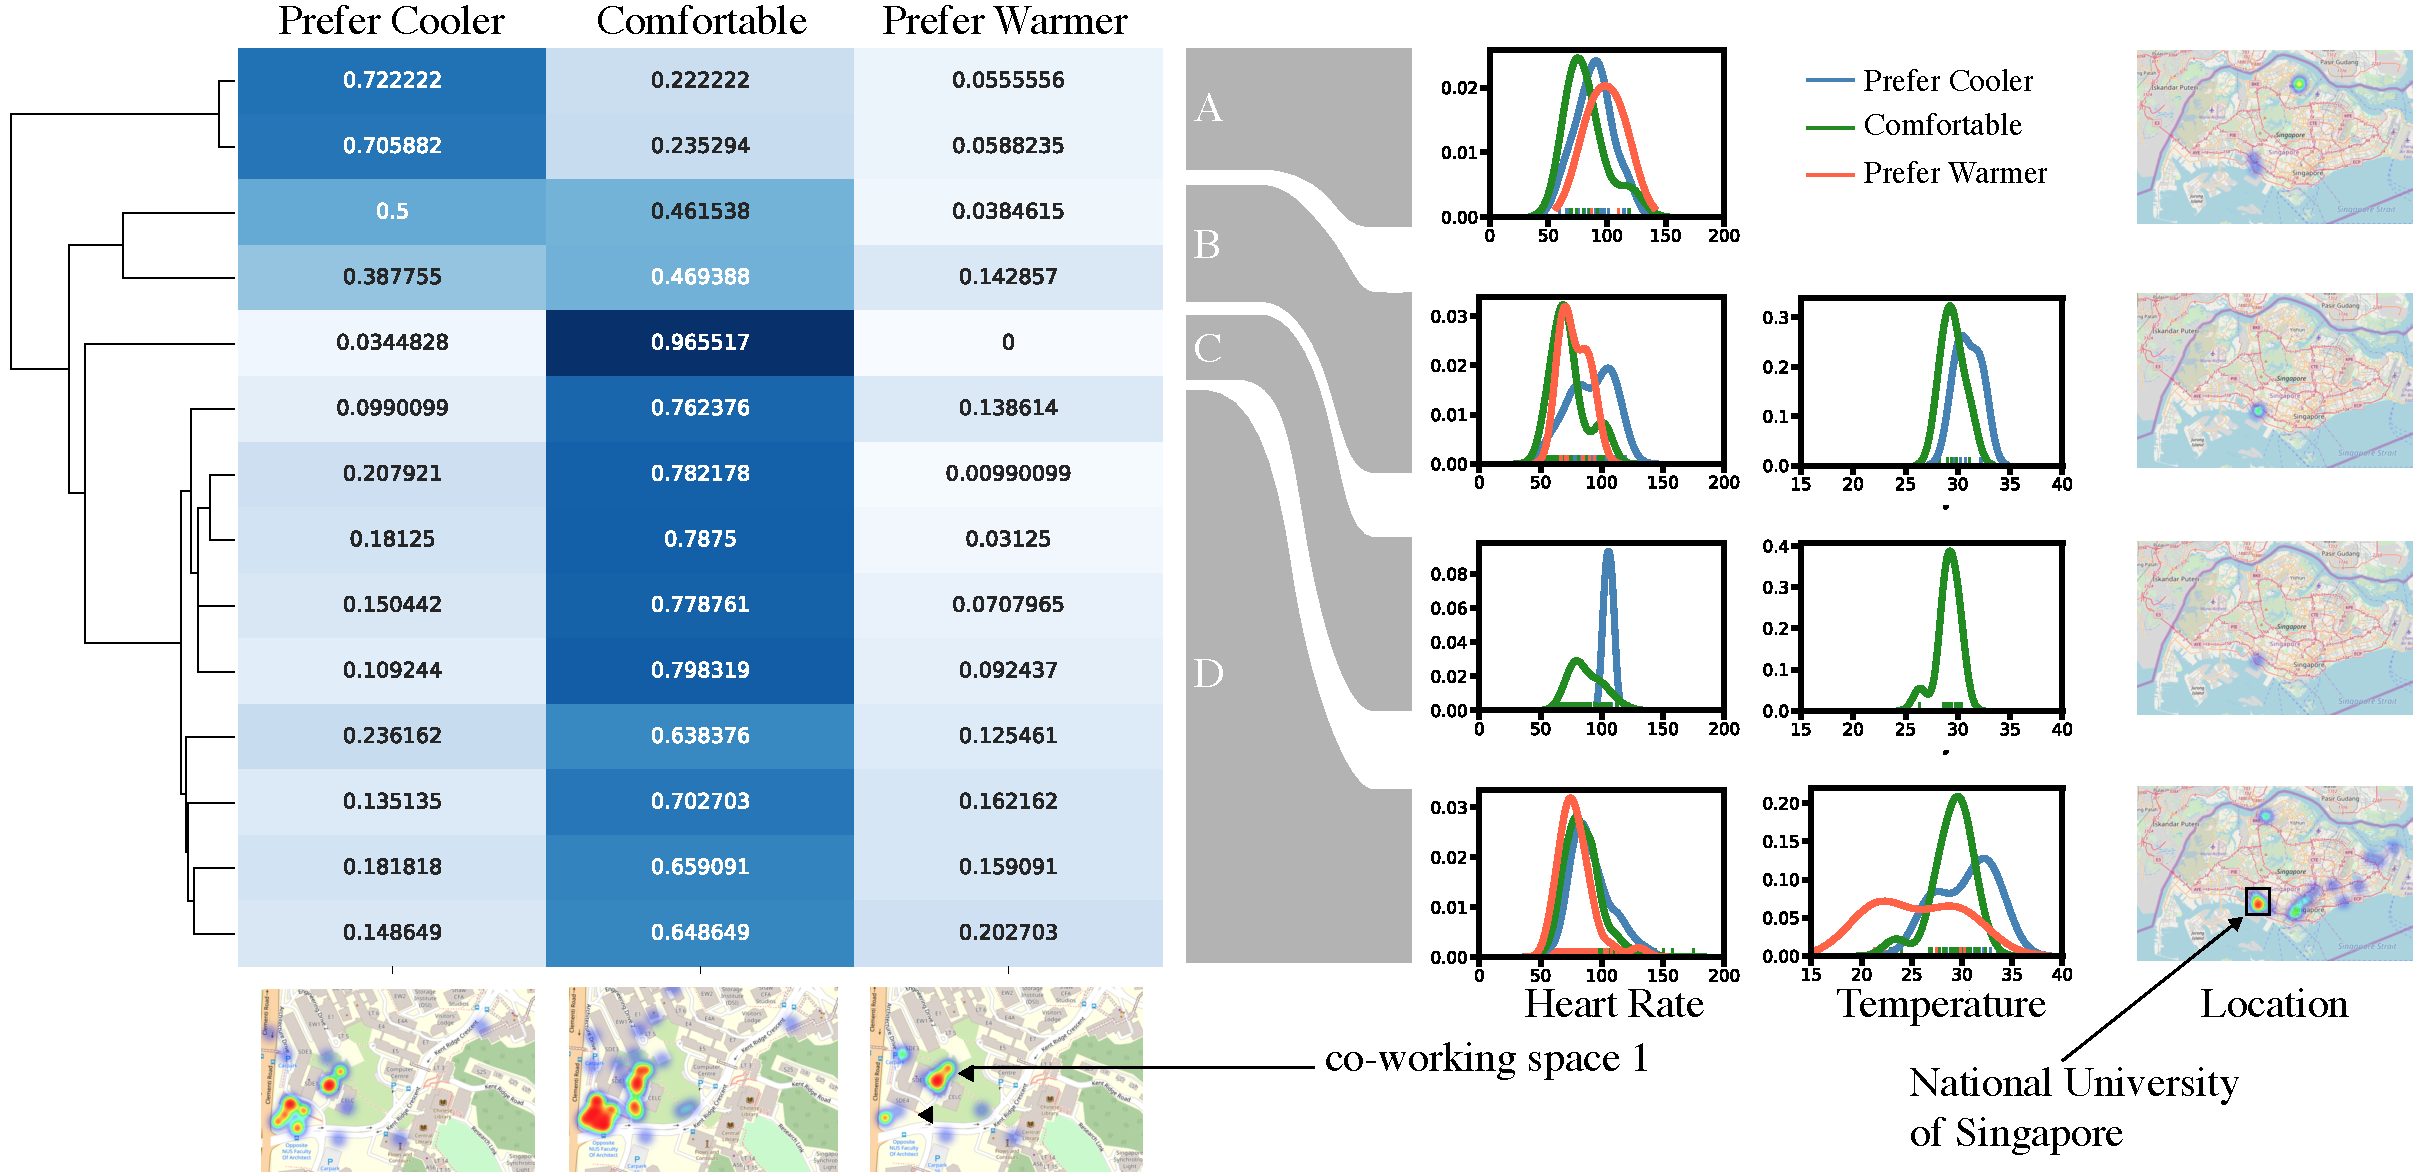
\includegraphics[width=\textwidth, trim= 0cm 0cm 0cm 0cm,clip]{cluster_results_compressed.pdf}
\caption{Heiracheal cluster-map of user feedback using k-means with euclidean distance. The numbers within the cluster-map detail the normalised number of responses. Four distinct groups can be observed. (A) two users that generally prefer cooler environments to their norm, (B) users that are comfortable 50\% of the time, (C) user that is almost always comfortable, (D) users that are comfortable on average 70\% of the time. To the right are breakdowns of the respective groups via sensor data and location. Below the cluster plot are spatial distributions of feedback responses at the university.}
\label{fig:clustering}
\end{center}
\end{figure}


% \begin{figure}
%     \begin{subfigure}[t]{0.49\textwidth}  
%     \centering
%         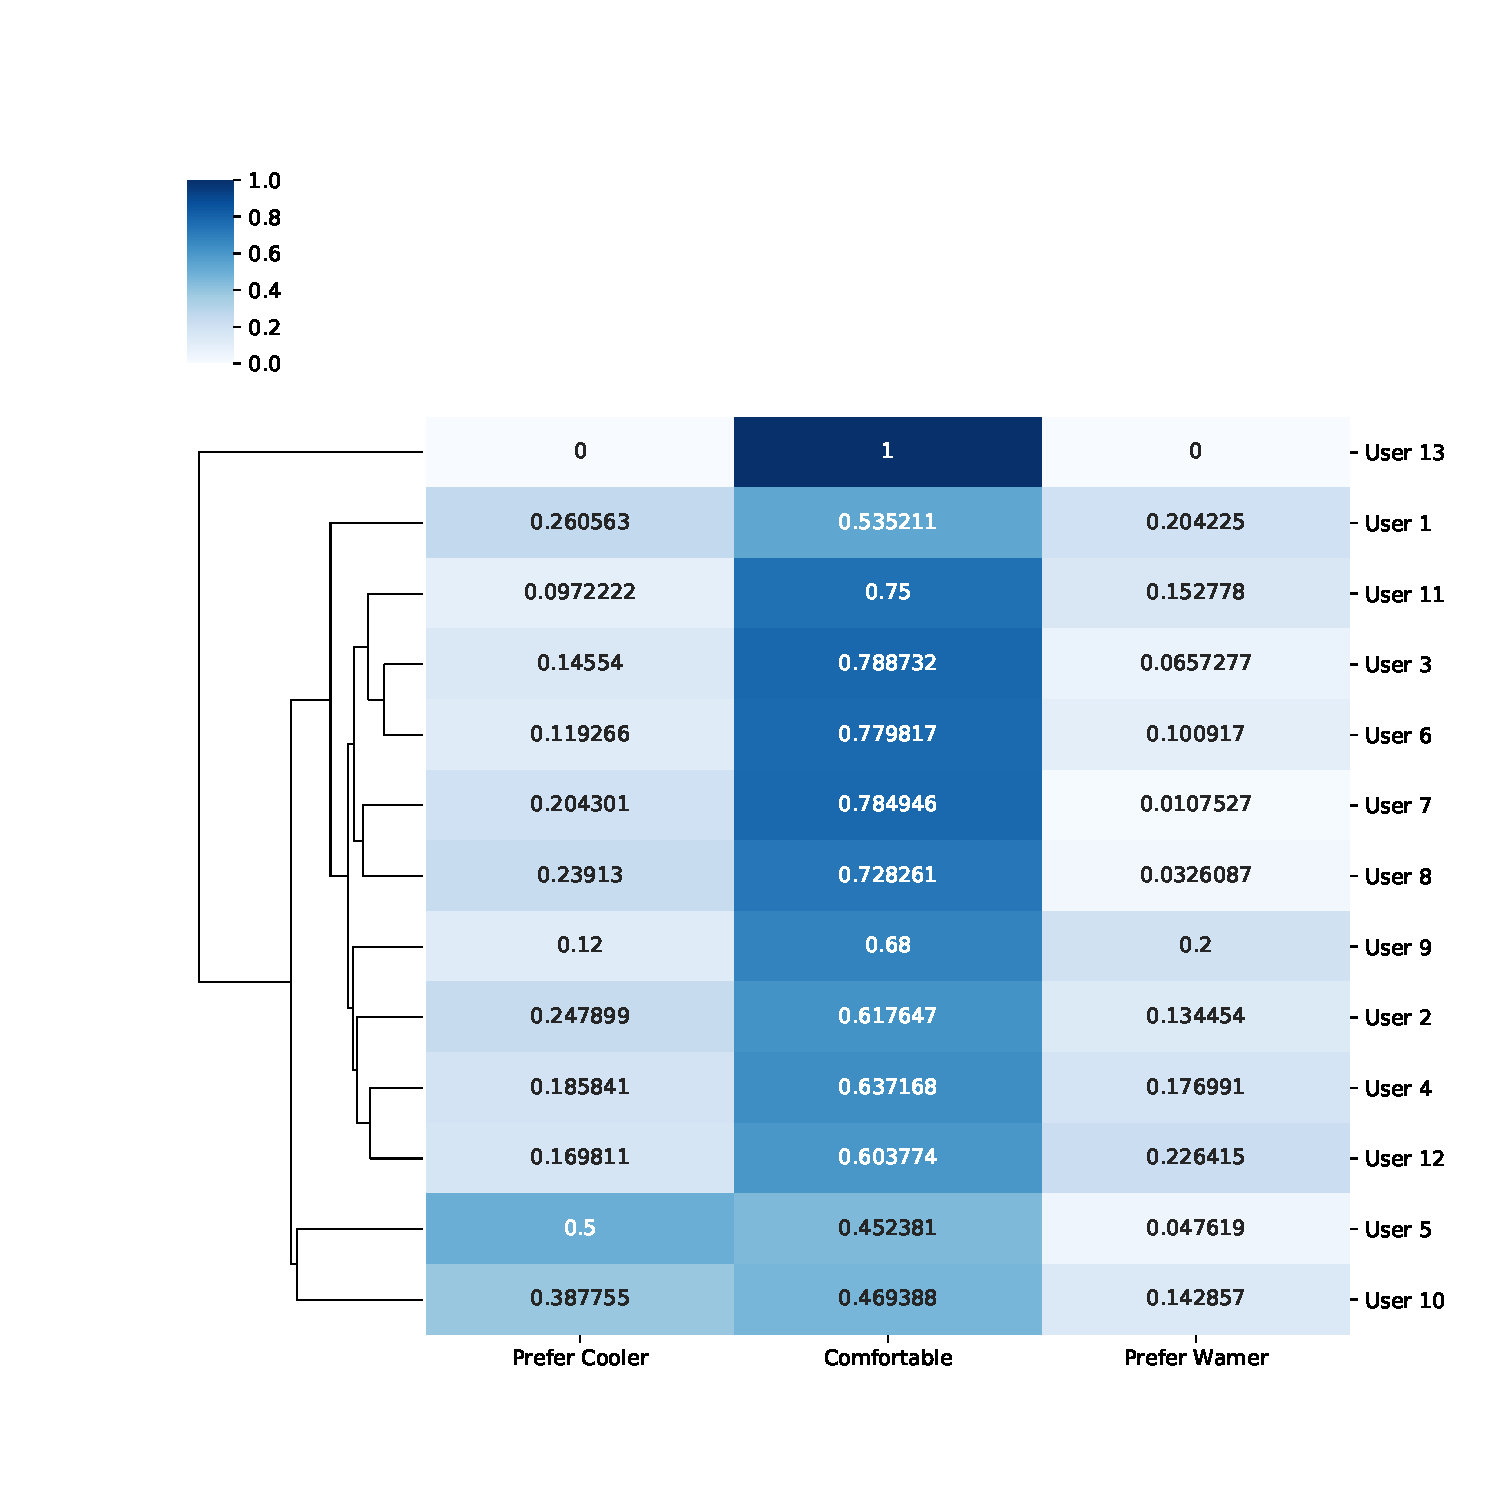
\includegraphics[width=\textwidth, trim= 0cm 0cm 0cm 0cm,clip]{cozie_users.pdf}
% 		\caption{(a)}
% 		\label{fig:userPlot}
%     \end{subfigure}
%     \begin{subfigure}[t]{0.49\textwidth}
%     \centering
%         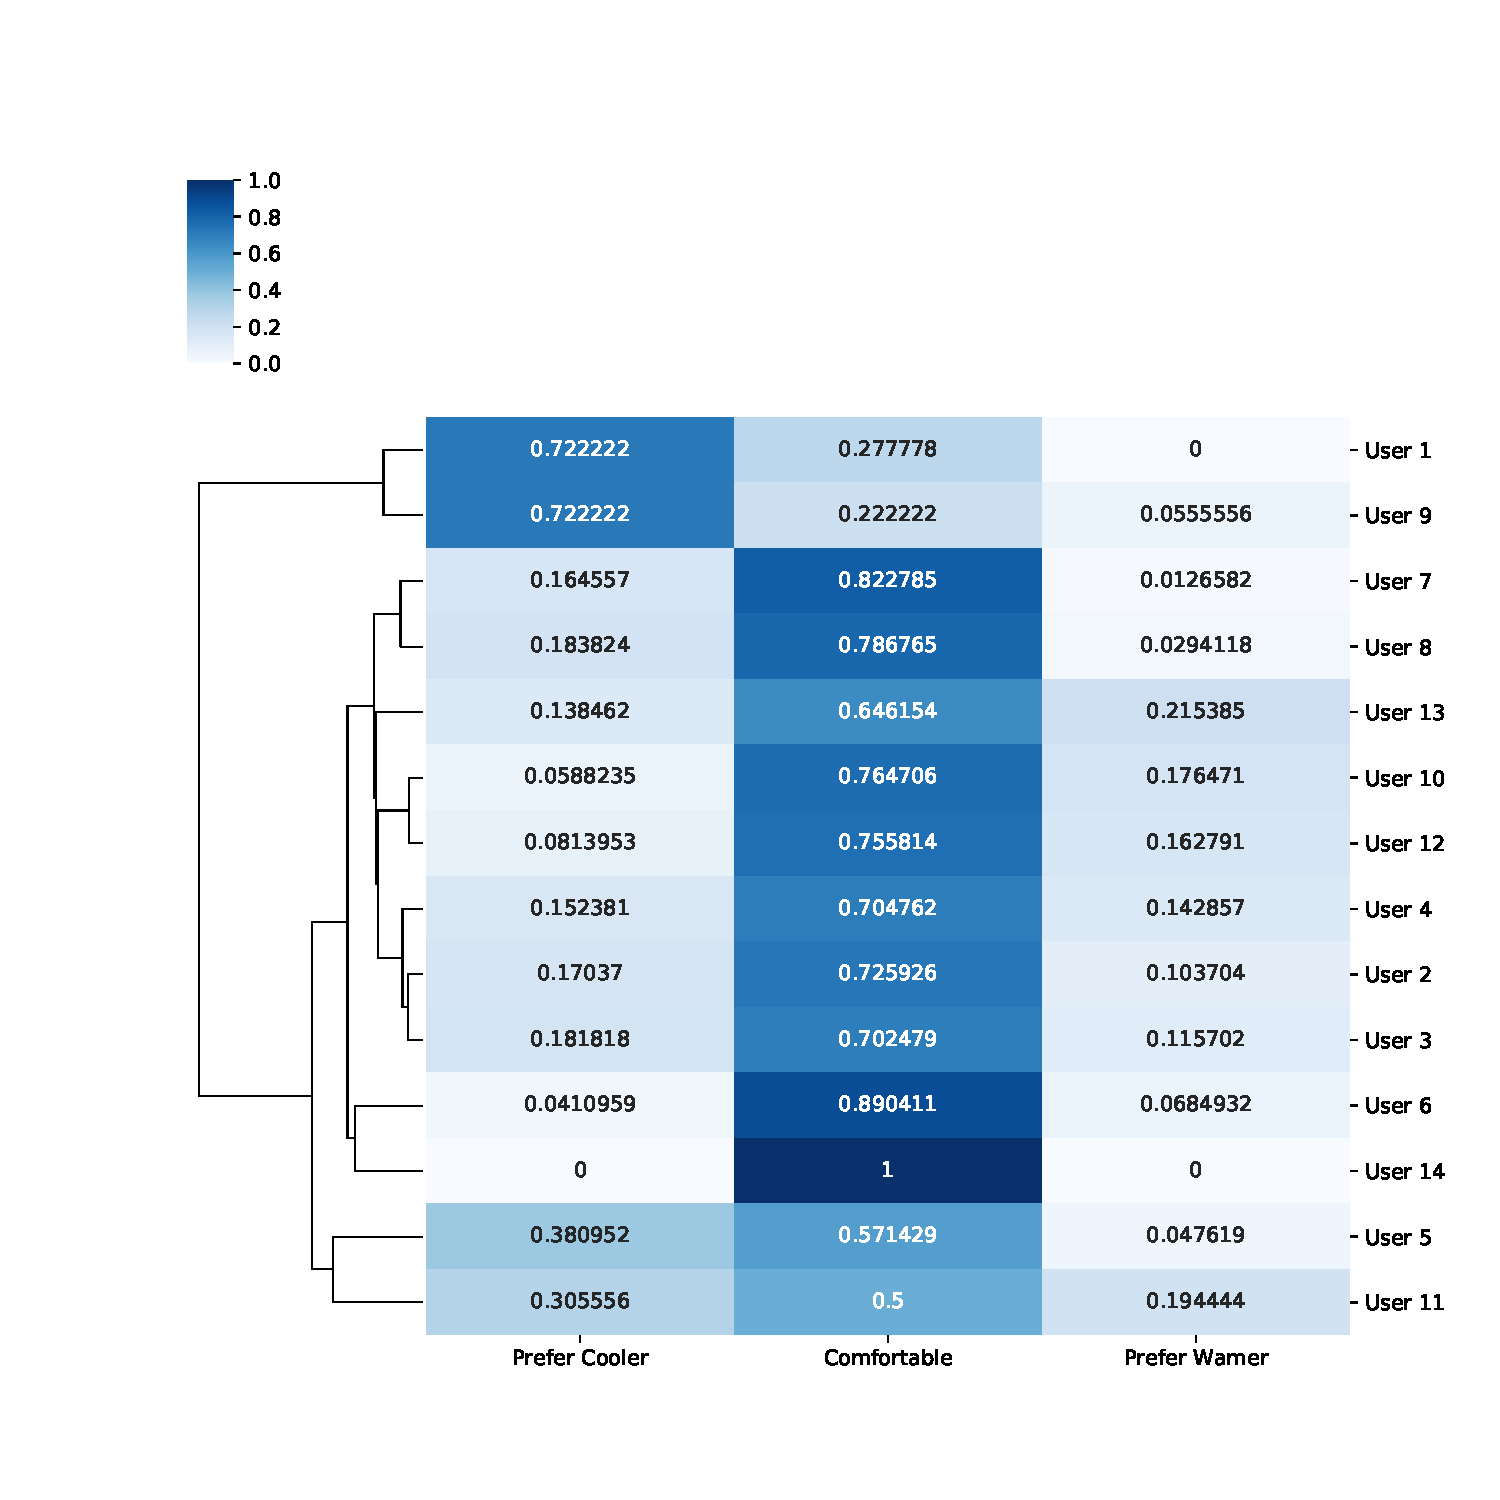
\includegraphics[width=\textwidth, trim= 0cm 0cm 0cm 0cm,clip]{cozie_users_lowheart.pdf}
% 		\caption{(b)}
% 		\label{fig:lowHeartUsers}
%     \end{subfigure}
%     \caption{Clustering of user feedback using hierarchal k-means. (a) The full results show four distinct clusters, (b) filter by heart rate that is less than 100 beats per minute}
%     \label{fig:clustering}
% \end{figure}




% \subsection{Influence of Heart-Rate}

% It is widely known that heart-rate influences metabolic activity, and therefore an occupants comfort preference. Figure \ref{fig:heartHist} details the number of responses for each thermal response based on the heart rate. [INSERT NUMBER HERE ] \% of "Prefer Cooler" responses occurred during higher metabolic activity when the heart rate was greater than 100 beats per minute. If we filter out these responses,and apply the same algorithms detailed in Section \ref{ch:userResults}, we see a slightly different response and clustering pattern, as shown in Figure \ref{fig:lowHeartUsers}. 



% \subsection{Combination with Sensor Data}




% convert time to bars
% one heart rate filter showing. Groups of similar behaving people. Group 1-4. What are the coincidental ranges of data belonging to these groups.

% \begin{figure}
% \centering
% 	\begin{subfigure}[t]{0.5\textwidth}
% 	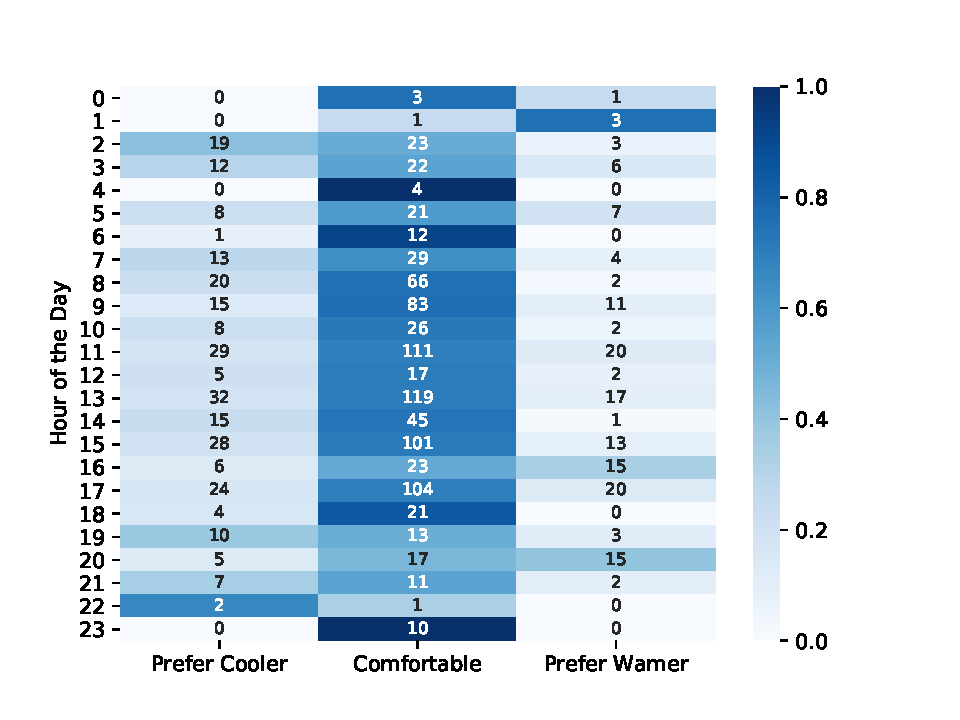
\includegraphics[width=\textwidth, trim= 0cm 0cm 0cm 0cm,clip]{hourPlot.pdf}
% 	\caption{(a)}
% 	\label{fig:hourPlot}
% 	\end{subfigure}
% 	\begin{subfigure}[t]{0.49\textwidth}
% 	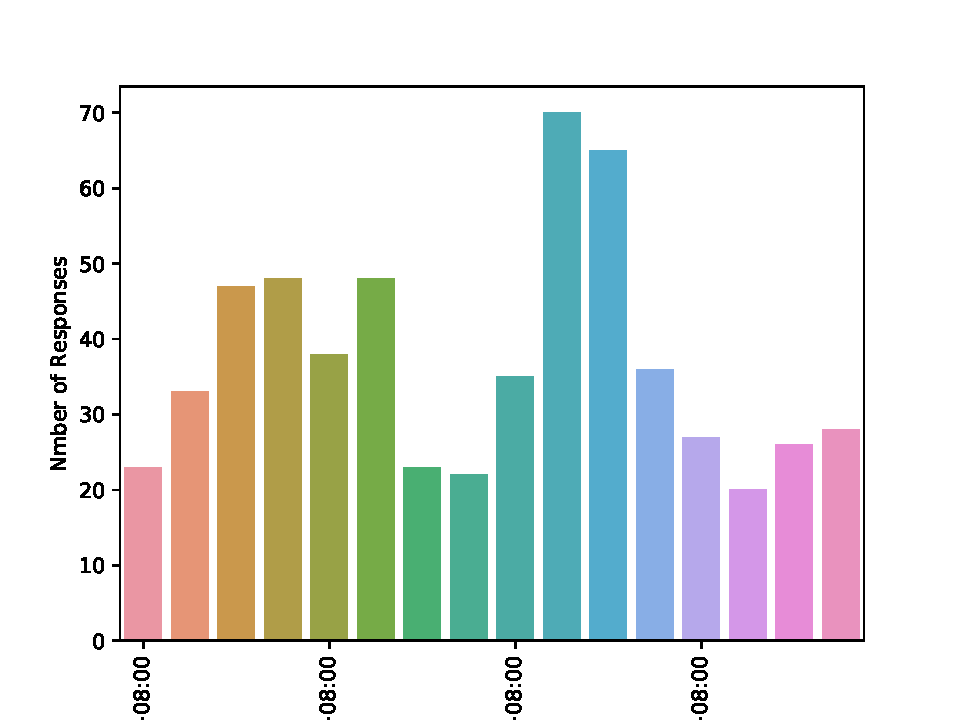
\includegraphics[width=\textwidth, trim= 0cm 0cm 0cm 0cm,clip]{response_rate.pdf}
% 	\caption{(b)}
% 	\label{fig:responseRate}
% 	\end{subfigure}
% 	\caption{(a) Aggregation of user feedback mapped to the hour of the day that feedback was given. Annotations within the heat-map detail the absolute response value, while the colour gradient relates to the normalised values (b) Daily responses during the course of the evaluation period. The dips in the graph are weekends}
% \end{figure}


% \begin{figure}
%     \centering
%     \begin{subfigure}[t]{0.3\textwidth}
%         \centering
%         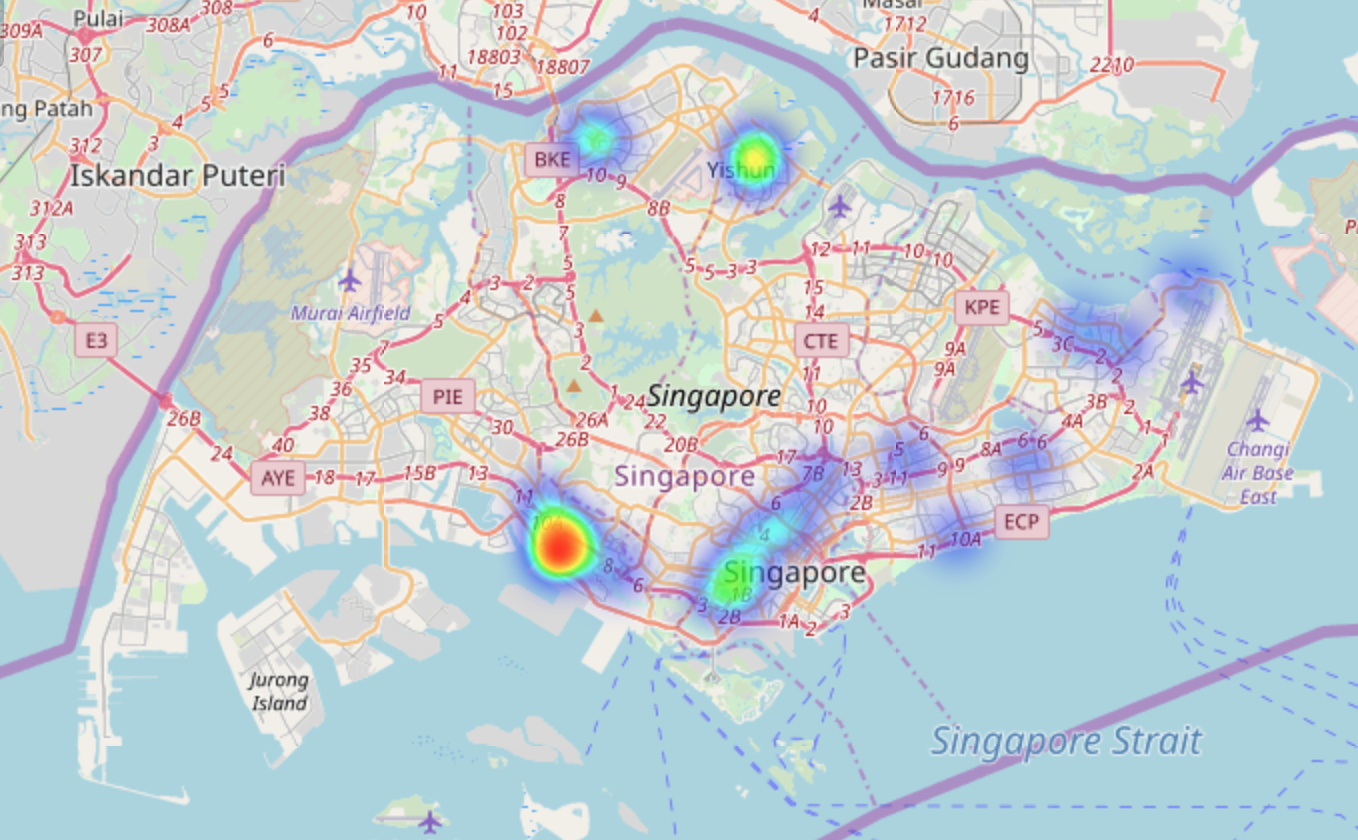
\includegraphics[height= 3cm]{map_singapore.png}
%         \caption{(a)}
%     \end{subfigure}
%     \begin{subfigure}[t]{0.3\textwidth}
%         \centering
%         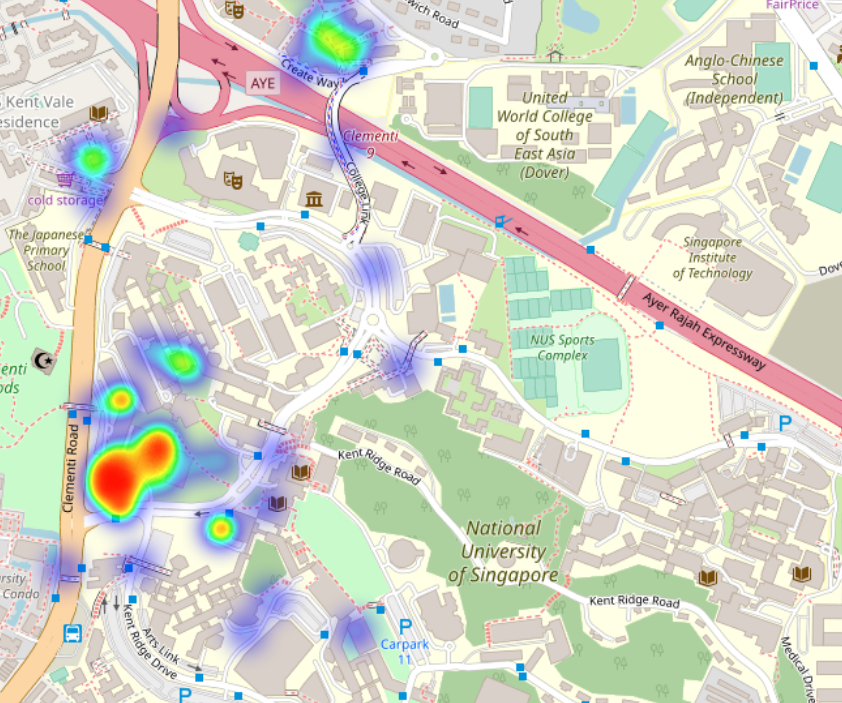
\includegraphics[height= 3cm]{map_nus.png}
%         \caption{(b)}
%     \end{subfigure}
%     \begin{subfigure}[t]{0.3\textwidth}
%         \centering
%         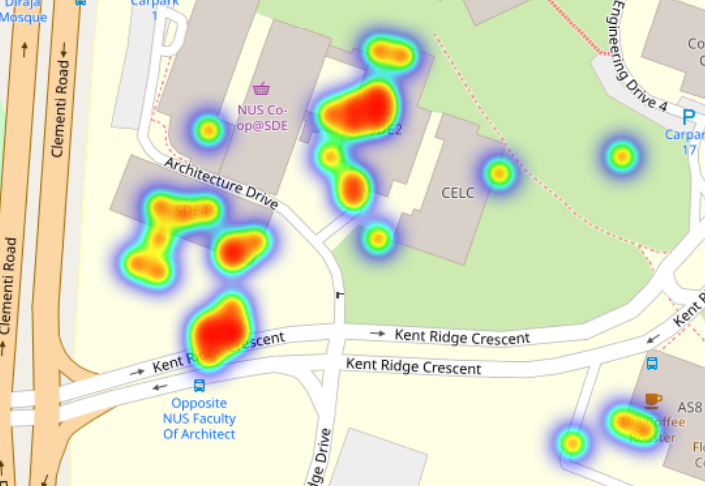
\includegraphics[height= 3cm]{map_sde.png}
%         \caption{(c)}
%     \end{subfigure}
%     \caption{Map of responses. From left to right, the city of Singapore, National University of Singapore, and the School of Design and Environment. The experiment was conducted at co-working spaces at the school of design and environment, however responses are seen throughout Singapore. Note that these results only show 634 of the [INSERT NUMBER] total responses as GPS localisation often failed indoors.}
%     \label{fig:map}
% \end{figure}



% \begin{figure}
%     \begin{subfigure}[t]{0.49\textwidth}  
%     \centering
% 	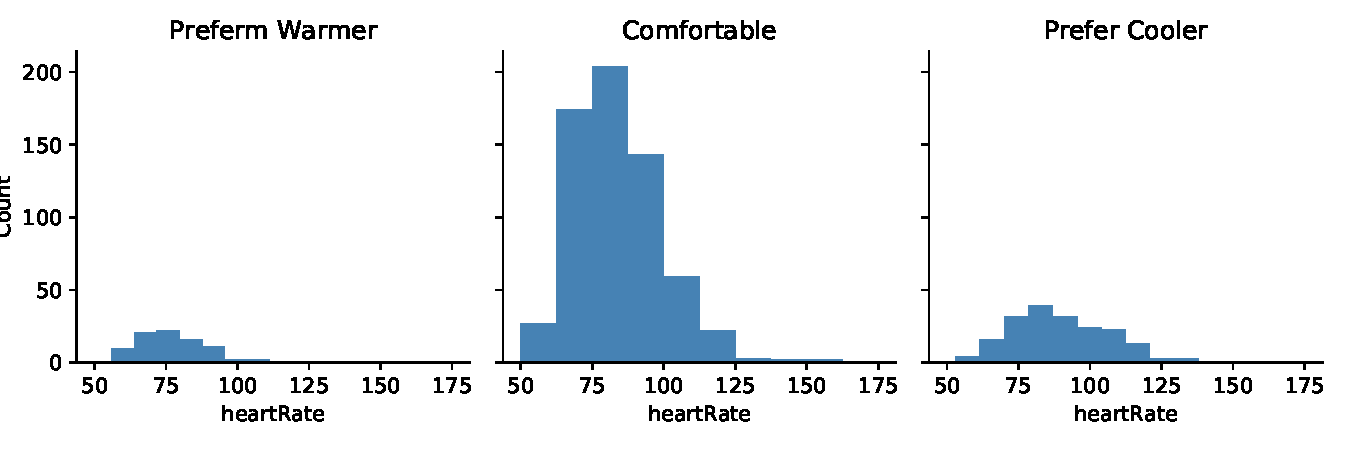
\includegraphics[width=\textwidth, trim= 0cm 0cm 0cm 0cm,clip]{heartHist.pdf}
% 	\caption{(a)}
% 	\label{fig:heartHist}
%     \end{subfigure}
%     \begin{subfigure}[t]{0.49\textwidth}
%     \centering
% 		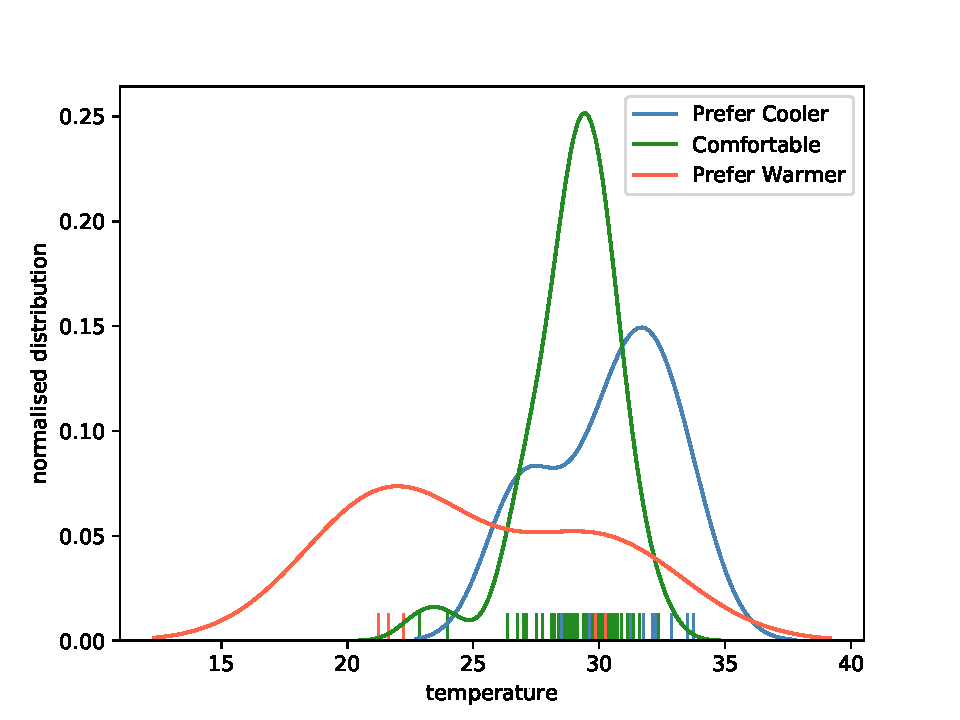
\includegraphics[width=\textwidth, trim= 0cm 0cm 0cm 0cm,clip]{temperatureHist.pdf}
% 		\caption{(b)}
% 		\label{fig:tempHist}	
%     \end{subfigure}
%     \caption{ Normalised distribution of the response type based on (a) heart rate (b) temperature. Note that the normalisation for "prefer warmer" is skewed due to the lack of responses of this type}
% \end{figure}


% \subsection{Evaluational of user comfort over a day}

% Figure \ref{fig:hourPlot} details a simple heat-map where the user comfort feedback is mapped to the hour of the day. Users appear to be comfortable on average [INSERT NUMEBR HERE] \% of the time, and there are no statistically significant trends during working hours (9:00 - 17:00). Variations in user comfort feedback during the day can be used to infer an issue within the building.

% It is interesting to note that there are more responses in the hours of 9:00, 11:00, 13:00, 15:00, and 17:00 when the occupant is buzzed and forced to give feedback. Nevertheless there are still significant amounts of responses made outside these times through the motivation of the participants themselves. Figure \ref{fig:summary}c details the daily responses from the participants, and no observable decrease in responses can be made. Dips in responses naturally occur during the weekend. 



% \section{Discussion}
% \label{ch:discussion}
% % !TEX root = 99_main.tex

\subsection{Large uncontrolled data vs. small controlled data}

%Let us take a step back and observe how market analysis was conducted. Traditionally, super markets would call individual households and ask for their feedback about what products they would like to have in stock. In modern times, applications such as facebook mine preference data from users based on what posts they "liked", and use this to generate targeted advertising for each individual.

%One can draw these parallels to human comfort surveying. 

Placing a group of participants in a controlled experimental space and conducting feedback surveys is a trusted traditional method for human comfort surveys. Giving each participant a smartwatch, and analysing the patterns of hundreds of data points per user would be more akin to modern data analytics employed in industries outside the building sector. Both methods are useful for reaching different types of conclusions. The traditional method can derive conclusions such as: \emph{4 of the 15 users felt warm at temperatures higher than 25.6 $^\circ$C}. This insight is useful in the context of the previously mentioned generalizable thermal comfort models that are traditionally created in built environment research, but have poor accuracy. On the other hand, the uncontrolled, large data method can draw conclusions such as: \emph{4 of 15 users can be categorized as a user type that prefers cooler working environments}. This paper focuses on the use of clustering to show the groups of \emph{comfort personality types}.

% that correspond with different behaviour in giving feedback and interacting with the spaces. 


%To further add to this, the uncontrolled method has minimal management overhead, and can be scaled by purchasing more devices, thus providing an even richer data set along the user axis. 

\subsection{In-situ benefits and limitations}
Uncontrolled experiments have minimal management overhead, which means that it can be easily scaled to larger groups by purchasing more devices. Furthermore, the users are analysed in their natural work environments and give feedback with a simple click on their watch. This reduction of effort results in no fatigue in the number of voluntary responses given as shown in Figure \ref{fig:summary}c. While users generally work from their office, they sometimes work from home, or at a local cafe. This presents a limitation in the context of traditional small controlled data. Large enough data must be obtained to filter out these scenarios and interpret meaningful results.


%The cozie watch face enables users to be analysed in-situ. By this we mean that the users work in their natural work environment, and give feedback with minimal effort. This allows the experiments to be conducted and scaled with minimal management overhead and there is no observable drop in voluntary responses in Figure \ref{fig:responseRate}. 

%there is no observable decrease in the feedback given. In fact, some of the users have enjoyed owning a fitbit, and will keep the device provided that they keep the cozie clock-face.\\


%With larger samples however, this uncontrolled situation presents an opportunity to better understand the behavioral characteristics of a user as certain patterns can be derived and interpreted. 

%If the research manager would like to have more control of the experiment they may choose to also add the "In Office / Out of Office" or the "Indoor/Outdoor" question to the list of questions asked.


%Placing participants in a controlled space and conducting surveys is a common and trusted method for human comfort research. In this methodology, users are under no control, and work from a designated co-working space at their own will, and at their own time. 


%One method commonly employed in comfort research involves placing a sample of participants in a controlled space and conducting surveys during this time. In this methodology, users are under no control. They are generally asked to work from the SDE4 building, however no direct restrictions are placed, and they are free to move as they like. (talk more about statistical significance of larger datasets and types of results infered )



\subsection{Indoor Localisation}
\label{ch:localisation}

The clock-face collects GPS data from the Fitbit, however GPS data indoors is not always reliable, and often not accessible. Only 30\% of all data points were tagged with GPS data. The team is currently investigating other methods such as Bluetooth based localisation from Steerpath, and pattern matching of wearable sensor data to indoor sensors.

% [CITE JUN]
% [CITE SpaceMatch @Clayton]

% \subsection{Problems Encountered}

% During the course of the experiment two Fitbits were lost by the users. One was lost permanently, and the other was found at a later date. There were also some issues with the collection of the environmental sensor data, resulting in only 79 matching points of the comfort feedback to the sensors, where as we expected approximately 200 matching points.







\section{Discussion and Conclusion}
\label{ch:conclusion}
% !TEX root = 99_main.tex

First trial runs of the cozie application for occupant comfort data collection have proven successful. Within just four weeks 1460 data points of thermal comfort were obtained from the 15 test participants, with minimal administrative overhead. This rich data set provides new opportunities in analysing occupant comfort behaviour through data driven methods. Within this paper, we have demonstrated how the data can be manipulated and clustered to group people into various comfort profiles. In our case there were 4 distinct groups, which can be then recommended spaces that better suit their comfort profile. The data can also be clustered via time to display building defects, or anomalies in occupant behaviour. Finally, we demonstrate how the app can be combined with wearable environmental sensors to cross reference a users preference to the environment that they were in. The watch-face is publicly available for download for use by researchers around the world.

Next steps in this research involve using cozie for the exploration of occupant clustering and spatial recommendation. We will explore elements of sound, light, and thermal comfort to determine whether spatial recommendation can serve as an alternative to individualised adaptive buildings control. Furthermore, the development of a \emph{strap-pack}, a smart-watch environmental sensor that can be adapted to the watch strap is underway. 

% \section{Acknowledgments}
% \label{ch:acknowledgments}
% % !TEX root = 99_main.tex

The authors would like to acknowledge the HiLo and HoNR project members for the design and construction of the ASF: Supermanoeuvre (Sydney Australia) and the Professorship of Architecture and Structures (BRG, ETH Zurich) for their work in designing the HiLo building; and the Institute of Structural Engineering (IBK, ETH Zurich) for their work in designing the HoNR building. The authors would also like to thank other key contributors to the ASF Project: Bratislav Svetozarevic, Moritz Begle, Stefan Caranovic. \\

This research was partly funded by the Climate-KIC, Building Technologies Accelerator program.


% \begin{appendices}
%  \label{ch:appendix}
%  % !TEX root = 99_main.tex

%  \end{appendices}

%% appendix sections are then done as normal sections
%% \appendix
%% \section{}
%% \label{}

%% bibitems, please use
\clearpage %to prevent figures from coming before the bib
  \bibliographystyle{elsarticle-num} 
  \bibliography{references}

\end{document}
\endinput
